\section{Design of the Controller}\label{designController}
The design of the controller is based on the Root Locus plot, where the final location of the poles in closed loop can be seen. Their position will depend on the different poles, zeros and gain of the controller and that is used to move them to a stable and better location.

The root locus of the system can be seen in \figref{rlocusCubli2}.

\begin{figure}[H]
	\centering 
	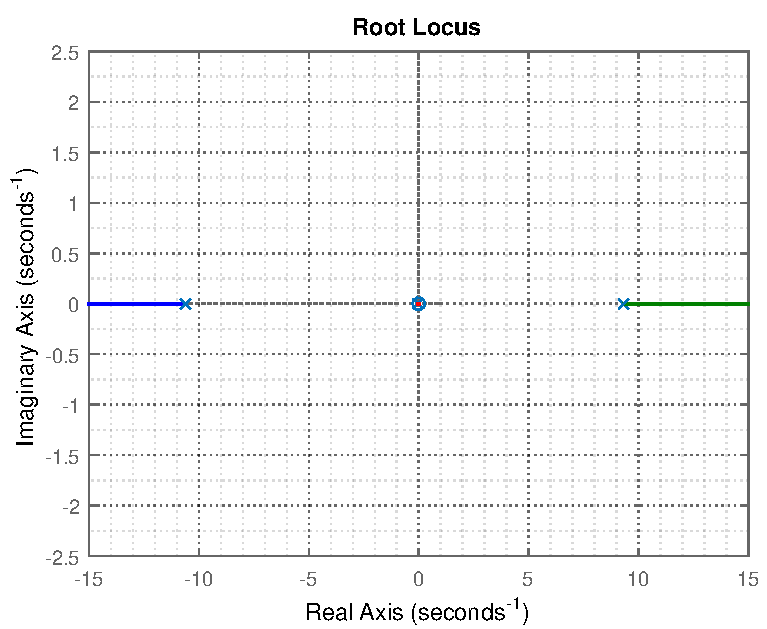
\includegraphics[scale=.56]{figures/rlocusCubli}
 	\captionof{figure}{Root Locus of the system}
 	\label{rlocusCubli2}
\end{figure}
%
As there exist one pole in the Right Half Plane (RHP), the controller must also have one there to create two branches which can be attracted to the Left Half Plane (LHP).

Then, two zeros must be placed in the LHP to make the branches enter in the stable region of the plot.

It is also important that the number of poles must be greater that the number of zeros for the controller to be feasible in reality. this means that two poles need to be placed somewhere so they don't affect the behavior of the final system. This can be achieve if they are placed in the LHP and far from the imaginary axis.

Finally, the gain must be adjusted to make the closed loop poles to be in a stable location. The resultant Root Locus can be seen in \figref{RLControllerZoom}.

\begin{figure}[H]
	\centering 
	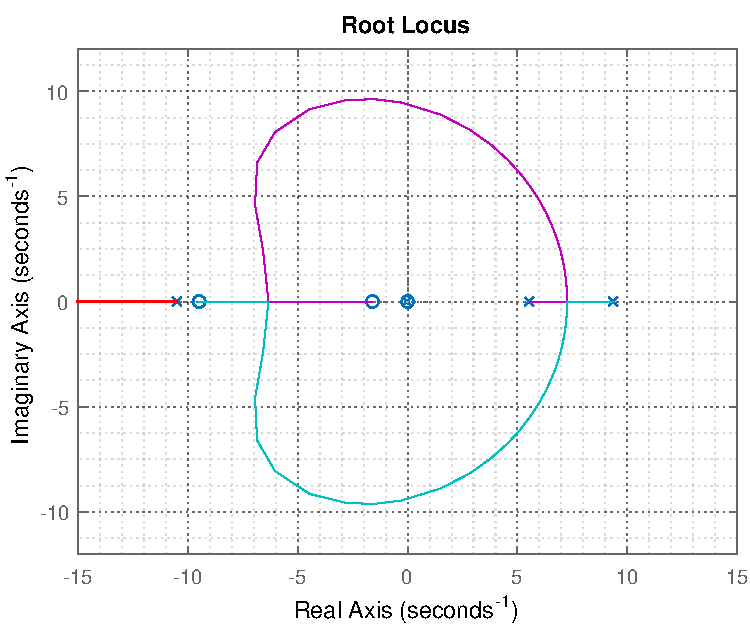
\includegraphics[scale=.56]{figures/RLControllerZoom}
	\captionof{figure}{Root Locus of the final system}
	\label{RLControllerZoom}
\end{figure}
%
The equation of final controller is then given by \eqref{ControllerLaplace}.

\begin{flalign}
	\eq{D(s)} {0,62737 \cdot \frac{(0,1054\ s + 1)\cdot (0,6254\ s + 1)}{(0,1805\ s - 1) \cdot (0,01\ s + 1) \cdot (0,005\ s + 1)}} & \nonumber\\
	\label{ControllerLaplace}
\end{flalign}
%
The stability of the controller given by \eqref{ControllerLaplace} can be then analyze using the Nyquist plot of the controller and the plant together, as seen in \figref{nyquistController}.

\begin{figure}[H] 
	\centering 
	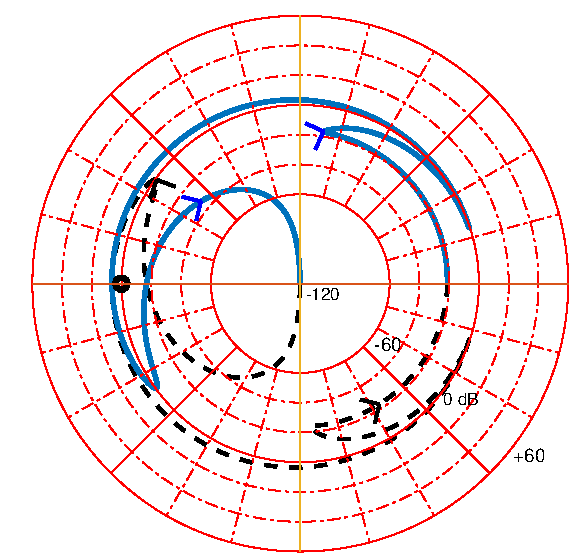
\includegraphics[scale=0.46]{figures/nyquistController}	
	\caption{Nyquist plot of the system with the controller}
	\label{nyquistController}
\end{figure}

Now the number of poles in the RHP is two and the number of encirclements around -1 is equals -2 (they are counterclockwise). This means that the system is stable, as the number of zeros in the RHP becomes 0.